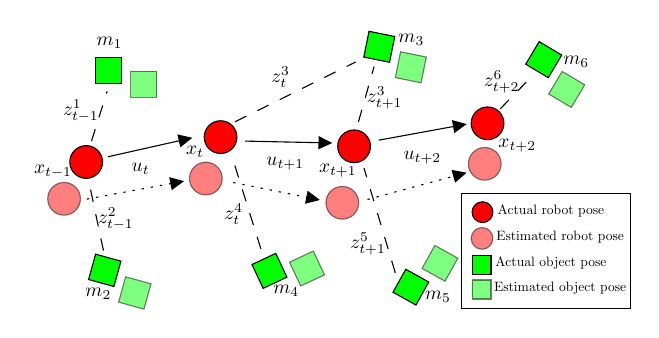
\begin{tikzpicture}[x=0.70pt,y=0.70pt,yscale=-0.60,xscale=0.60, every node/.style={scale=0.70}]
%uncomment if require: \path (0,258); %set diagram left start at 0, and has height of 258

%Shape: Ellipse [id:dp7434301091862943] 
\draw  [color=black  ,draw opacity=0.5 ][fill=red  ,fill opacity=0.5 ] (6.44,153.49) .. controls (6.44,145.72) and (12.74,139.42) .. (20.52,139.42) .. controls (28.29,139.42) and (34.6,145.72) .. (34.6,153.49) .. controls (34.6,161.27) and (28.29,167.57) .. (20.52,167.57) .. controls (12.74,167.57) and (6.44,161.27) .. (6.44,153.49) -- cycle ;
%Shape: Rectangle [id:dp6808133197576726] 
\draw  [color=black  ,draw opacity=1 ][fill=green  ,fill opacity=1 ] (47.63,31.7) -- (70.24,31.7) -- (70.24,54.31) -- (47.63,54.31) -- cycle ;
%Shape: Ellipse [id:dp13056961037551362] 
\draw  [color=black  ,draw opacity=0.5 ][fill=red  ,fill opacity=0.5 ] (128.41,136.07) .. controls (128.41,128.29) and (134.72,121.99) .. (142.49,121.99) .. controls (150.27,121.99) and (156.57,128.29) .. (156.57,136.07) .. controls (156.57,143.84) and (150.27,150.15) .. (142.49,150.15) .. controls (134.72,150.15) and (128.41,143.84) .. (128.41,136.07) -- cycle ;
%Shape: Ellipse [id:dp9996445403573203] 
\draw  [color=black  ,draw opacity=0.5 ][fill=red  ,fill opacity=0.5 ] (245.81,156.91) .. controls (245.81,149.13) and (252.11,142.83) .. (259.89,142.83) .. controls (267.66,142.83) and (273.97,149.13) .. (273.97,156.91) .. controls (273.97,164.68) and (267.66,170.99) .. (259.89,170.99) .. controls (252.11,170.99) and (245.81,164.68) .. (245.81,156.91) -- cycle ;
%Shape: Ellipse [id:dp1885221377208316] 
\draw  [color=black  ,draw opacity=0.5 ][fill=red  ,fill opacity=0.5 ] (368.4,123.4) .. controls (368.4,115.62) and (374.7,109.32) .. (382.48,109.32) .. controls (390.25,109.32) and (396.55,115.62) .. (396.55,123.4) .. controls (396.55,131.17) and (390.25,137.47) .. (382.48,137.47) .. controls (374.7,137.47) and (368.4,131.17) .. (368.4,123.4) -- cycle ;
%Shape: Ellipse [id:dp5392362763171864] 
\draw  [fill=red  ,fill opacity=1 ] (25.45,121.81) .. controls (25.45,114.04) and (31.75,107.73) .. (39.53,107.73) .. controls (47.3,107.73) and (53.61,114.04) .. (53.61,121.81) .. controls (53.61,129.59) and (47.3,135.89) .. (39.53,135.89) .. controls (31.75,135.89) and (25.45,129.59) .. (25.45,121.81) -- cycle ;
%Shape: Ellipse [id:dp9130435739184759] 
\draw  [fill=red  ,fill opacity=1 ] (141.09,100.43) .. controls (141.09,92.65) and (147.39,86.35) .. (155.16,86.35) .. controls (162.94,86.35) and (169.24,92.65) .. (169.24,100.43) .. controls (169.24,108.2) and (162.94,114.51) .. (155.16,114.51) .. controls (147.39,114.51) and (141.09,108.2) .. (141.09,100.43) -- cycle ;
%Shape: Ellipse [id:dp11001638797843405] 
\draw  [fill=red  ,fill opacity=1 ] (255.93,108.35) .. controls (255.93,100.57) and (262.23,94.27) .. (270.01,94.27) .. controls (277.78,94.27) and (284.09,100.57) .. (284.09,108.35) .. controls (284.09,116.12) and (277.78,122.43) .. (270.01,122.43) .. controls (262.23,122.43) and (255.93,116.12) .. (255.93,108.35) -- cycle ;
%Shape: Ellipse [id:dp21523771226438004] 
\draw  [fill=red  ,fill opacity=1 ] (370.77,88.55) .. controls (370.77,80.77) and (377.08,74.47) .. (384.85,74.47) .. controls (392.63,74.47) and (398.93,80.77) .. (398.93,88.55) .. controls (398.93,96.32) and (392.63,102.63) .. (384.85,102.63) .. controls (377.08,102.63) and (370.77,96.32) .. (370.77,88.55) -- cycle ;
%Shape: Rectangle [id:dp39352313397759164] 
\draw  [color=black  ,draw opacity=0.5 ][fill=green  ,fill opacity=0.5 ] (77.72,43.58) -- (100.34,43.58) -- (100.34,66.19) -- (77.72,66.19) -- cycle ;
%Shape: Rectangle [id:dp10940816352865923] 
\draw  [color=black  ,draw opacity=1 ][fill=green  ,fill opacity=1 ] (47.64,201.12) -- (69.44,207.16) -- (63.4,228.95) -- (41.61,222.91) -- cycle ;
%Shape: Rectangle [id:dp45450106813081703] 
\draw  [color=black  ,draw opacity=0.5 ][fill=green  ,fill opacity=0.5 ] (73.48,220.6) -- (95.27,226.64) -- (89.23,248.43) -- (67.44,242.4) -- cycle ;
%Shape: Rectangle [id:dp2630909080760764] 
\draw  [color=black  ,draw opacity=1 ][fill=green  ,fill opacity=1 ] (182.2,210.05) -- (202.67,200.45) -- (212.27,220.93) -- (191.79,230.52) -- cycle ;
%Shape: Rectangle [id:dp7021199786756188] 
\draw  [color=black  ,draw opacity=0.5 ][fill=green  ,fill opacity=0.5 ] (214.49,208.03) -- (234.97,198.44) -- (244.56,218.91) -- (224.09,228.51) -- cycle ;
%Shape: Rectangle [id:dp8406498517381461] 
\draw  [color=black  ,draw opacity=1 ][fill=green  ,fill opacity=1 ] (282.86,9.37) -- (305.02,13.87) -- (300.52,36.03) -- (278.36,31.53) -- cycle ;
%Shape: Rectangle [id:dp5992753478320311] 
\draw  [color=black  ,draw opacity=0.5 ][fill=green  ,fill opacity=0.5 ] (309.99,27.01) -- (332.15,31.51) -- (327.65,53.67) -- (305.49,49.17) -- cycle ;
%Shape: Rectangle [id:dp48388398423368595] 
\draw  [color=black  ,draw opacity=0.5 ][fill=green  ,fill opacity=0.5 ] (359.28,204.6) -- (348.28,224.35) -- (328.52,213.35) -- (339.52,193.6) -- cycle ;
%Shape: Rectangle [id:dp44335535839655893] 
\draw  [color=black  ,draw opacity=1 ][fill=green  ,fill opacity=1 ] (334.26,225.11) -- (323.26,244.87) -- (303.5,233.87) -- (314.5,214.11) -- cycle ;
%Shape: Rectangle [id:dp2110614236699101] 
\draw  [color=black  ,draw opacity=1 ][fill=green  ,fill opacity=1 ] (429.25,18.27) -- (448.67,29.84) -- (437.11,49.27) -- (417.68,37.7) -- cycle ;
%Shape: Rectangle [id:dp734525975812425] 
\draw  [color=black  ,draw opacity=0.5 ][fill=green  ,fill opacity=0.5 ] (449.03,43.87) -- (468.46,55.44) -- (456.89,74.87) -- (437.46,63.3) -- cycle ;
%Straight Lines [id:da8771117550774294] 
\draw    (58.36,117.3) -- (126.9,101.9) ;
\draw [shift={(128.85,101.46)}, rotate = 527.3299999999999] [fill={rgb, 255:red, 0; green, 0; blue, 0 }  ][line width=0.75]    (8.93,-4.29) -- (0,0) -- (8.93,4.29) -- cycle    ;

%Straight Lines [id:da7204140282863669] 
\draw  [dash pattern={on 0.84pt off 2.51pt}]  (40.14,153.74) -- (119.75,139.05) ;
\draw [shift={(121.72,138.69)}, rotate = 529.55] [fill={rgb, 255:red, 0; green, 0; blue, 0 }  ][line width=0.75]    (8.93,-4.29) -- (0,0) -- (8.93,4.29) -- cycle    ;

%Straight Lines [id:da8591492656423307] 
\draw    (176.37,103.84) -- (247.24,105.38) ;
\draw [shift={(249.24,105.42)}, rotate = 181.25] [fill={rgb, 255:red, 0; green, 0; blue, 0 }  ][line width=0.75]    (8.93,-4.29) -- (0,0) -- (8.93,4.29) -- cycle    ;

%Straight Lines [id:da09058967319467015] 
\draw  [dash pattern={on 0.84pt off 2.51pt}]  (166.07,139.48) -- (236.59,153.69) ;
\draw [shift={(238.55,154.08)}, rotate = 191.39] [fill={rgb, 255:red, 0; green, 0; blue, 0 }  ][line width=0.75]    (8.93,-4.29) -- (0,0) -- (8.93,4.29) -- cycle    ;

%Straight Lines [id:da6287850967405952] 
\draw    (291.21,103.05) -- (362.91,89.94) ;
\draw [shift={(364.87,89.58)}, rotate = 529.64] [fill={rgb, 255:red, 0; green, 0; blue, 0 }  ][line width=0.75]    (8.93,-4.29) -- (0,0) -- (8.93,4.29) -- cycle    ;

%Straight Lines [id:da39601612623948923] 
\draw  [dash pattern={on 0.84pt off 2.51pt}]  (281.55,154.08) -- (362.94,132.08) ;
\draw [shift={(364.87,131.56)}, rotate = 524.87] [fill={rgb, 255:red, 0; green, 0; blue, 0 }  ][line width=0.75]    (8.93,-4.29) -- (0,0) -- (8.93,4.29) -- cycle    ;

%Straight Lines [id:da14218951162996163] 
\draw  [dash pattern={on 4.5pt off 4.5pt}]  (44.1,103.84) -- (57.57,61.07) ;


%Straight Lines [id:da5099949144358528] 
\draw  [dash pattern={on 4.5pt off 4.5pt}]  (54.4,198.09) -- (42.52,141.86) ;


%Straight Lines [id:da8152861145371411] 
\draw  [dash pattern={on 4.5pt off 4.5pt}]  (167.66,87.21) -- (271.41,35.73) ;


%Straight Lines [id:da6504983020328421] 
\draw  [dash pattern={on 4.5pt off 4.5pt}]  (273.79,87.21) -- (287.25,39.69) ;


%Straight Lines [id:da09932466850869759] 
\draw  [dash pattern={on 4.5pt off 4.5pt}]  (189.83,196.51) -- (166.07,120.47) ;


%Straight Lines [id:da5252262954209137] 
\draw  [dash pattern={on 4.5pt off 4.5pt}]  (305.47,217.1) -- (278.55,127.08) ;


%Straight Lines [id:da11641625781770915] 
\draw  [dash pattern={on 4.5pt off 4.5pt}]  (395.76,76.12) -- (423.48,47.61) ;


%Shape: Rectangle [id:dp779804859980624] 
\draw   (362.5,148.99) -- (507.55,148.99) -- (507.55,247.99) -- (362.5,247.99) -- cycle ;
%Shape: Circle [id:dp9912886474851581] 
\draw  [fill=red  ,fill opacity=1 ] (371.57,164.98) .. controls (371.57,160.05) and (375.56,156.05) .. (380.5,156.05) .. controls (385.43,156.05) and (389.43,160.05) .. (389.43,164.98) .. controls (389.43,169.91) and (385.43,173.91) .. (380.5,173.91) .. controls (375.56,173.91) and (371.57,169.91) .. (371.57,164.98) -- cycle ;
%Shape: Ellipse [id:dp633215489310963] 
\draw  [color=black  ,draw opacity=0.5 ][fill=red  ,fill opacity=0.5 ] (370.77,187.55) .. controls (370.77,182.4) and (374.95,178.22) .. (380.1,178.22) .. controls (385.25,178.22) and (389.43,182.4) .. (389.43,187.55) .. controls (389.43,192.7) and (385.25,196.88) .. (380.1,196.88) .. controls (374.95,196.88) and (370.77,192.7) .. (370.77,187.55) -- cycle ;
%Shape: Square [id:dp9486488989130497] 
\draw  [color=black  ,draw opacity=1 ][fill=green  ,fill opacity=1 ] (371.57,201.99) -- (387.84,201.99) -- (387.84,218.26) -- (371.57,218.26) -- cycle ;
%Shape: Square [id:dp13355255501454244] 
\draw  [color=black  ,draw opacity=0.5 ][fill=green  ,fill opacity=0.5 ] (371.57,223.37) -- (387.84,223.37) -- (387.84,239.65) -- (371.57,239.65) -- cycle ;

% Text Node
\draw (10.98,129.95) node   {$\boldsymbol{x}_{t-1}$};
% Text Node
\draw (133.17,113.11) node   {$\boldsymbol{x}_{t}$};
% Text Node
\draw (256.02,129.53) node   {$\boldsymbol{x}_{t+1}$};
% Text Node
\draw (410.38,107.73) node   {$\boldsymbol{x}_{t+2}$};
% Text Node
\draw (86.44,127.53) node   {$\boldsymbol{u}_{t}$};
% Text Node
\draw (210.78,123.57) node   {$\boldsymbol{u}_{t+1}$};
% Text Node
\draw (328.8,118.03) node   {$\boldsymbol{u}_{t+2}$};
% Text Node
\draw (34.95,77.64) node   {$\boldsymbol{z}^{1}_{t-1}$};
% Text Node
\draw (65.05,171.1) node   {$\boldsymbol{z}^{2}_{t-1}$};
% Text Node
\draw (206.82,49.12) node   {$\boldsymbol{z}^{3}_{t}$};
% Text Node
\draw (166.43,166.34) node   {$\boldsymbol{z}^{4}_{t}$};
% Text Node
\draw (296.32,66.55) node   {$\boldsymbol{z}^{3}_{t+1}$};
% Text Node
\draw (282.07,192.48) node   {$\boldsymbol{z}^{5}_{t+1}$};
% Text Node
\draw (396.91,53.08) node   {$\boldsymbol{z}^{6}_{t+2}$};
% Text Node
\draw (59.51,19.03) node   {$\boldsymbol{m}_{1}$};
% Text Node
\draw (50,235.25) node   {$\boldsymbol{m}_{2}$};
% Text Node
\draw (319.29,16.65) node   {$\boldsymbol{m}_{3}$};
% Text Node
\draw (211.58,232.87) node   {$\boldsymbol{m}_{4}$};
% Text Node
\draw (342.26,237.63) node   {$\boldsymbol{m}_{5}$};
% Text Node
\draw (461.07,35.66) node   {$\boldsymbol{m}_{6}$};
% Text Node
\draw (439.34,163.97) node [scale=0.7] [align=left] {Actual robot pose};
% Text Node
\draw (447.34,186.14) node [scale=0.7] [align=left] {Estimated robot pose};
% Text Node
\draw (439.34,209.11) node [scale=0.7] [align=left] {Actual object pose};
% Text Node
\draw (447.34,230.5) node [scale=0.7] [align=left] {Estimated object pose};

\end{tikzpicture}